%!TEX root = ../main.tex

\section{Introduction}
 
Nowadays, the number of open datasets from multiple sources ($e.g.,$ governments and companies) keeps growing, which provides large potential opportunity for intelligent data analysis. However, these datasets are always stored in the data lake that are not well-organized like storing in a database with well-defined schemes and indexes. Hence, it is challenging to efficiently and effectively find user-required data considering the data lake scale and the semantics of user requirements.  
To exploit the enormous value in the data lake, researchers from both industry and academia have implemented a number of data discovery engines~\cite{} that retrieve relevant user-specified tables. 


%given a query table, they search relevant tables from the data lake, so as to benefit the downstream applications, such as augmenting more data instances~\cite{} or  improving the machine learning model performance~\cite{}. 

\begin{table*}[t]
	\centering
	\caption{Benchmark Comparison.}
	\begin{tabular}{|c|c|c|c|c|c|c|}
		\hline
		\centering
		Benchmarks & Type & $\#$-Query tables & $\#$-Lake tables & $\#$-Total columns & Size (GB) & Source  \\
		\hline
		TUS Small~\cite{TUS}& Union  & 200 & 1,530 & 14,810 & 1 & Open Data  \\
		\hline
		TUS Large~\cite{TUS}& Union  & 1,000 & 5,043 & 54,923 & 1.5 & Open Data  \\
		\hline
		Santos Small~\cite{Santos}& Union  & 50 & 550 & 6,322 & 0.45 & Open Data  \\
		\hline
		Santos Large~\cite{Santos}& Union  & 80 & 11,090 & 123,477 & 11 & Open Data  \\
		\hline
	\end{tabular}
	\label{Table:benchmarks}

\end{table*}

In general, discovering related tables from data lakes can be generally categorized into several sub-tasks, namely keyword-based search, joinable table search and unionable table search.
The first category~\cite{} issues keywords as queries, based on which relevant tables are retrieved. 
We focus on the latter two categories that issue a table as the query, which have recently attracted much attention because they are widely-used for augmenting more data instances~\cite{} or features~\cite{}, so as to  benefit the downstream applications like machine learning based data analysis.
%


To be specific, given a query table with a user-specified column, joinable table search finds the target tables that can be joined with the column.

\begin{example}
	As shown in Figure~\ref{fig:example}(a), given the query table ($T_1$) and a specified column \texttt{Corporation},  
	we can observe that Table $T_2$ in the data lake is joinable, \ie the first attribute of $T_2$ can be joined with the specified column mainly because i). the column names are  matching  and 
	ii). there exist a number of semantically overlapping cell values (\eg Apple and Apple Inc.). 
	%
	The joined table can be taken as feature augmentation to improve model performance when  the \texttt{Price} is treated as the predicted column. 
	%
	In addition, although the first attribute of $T_3$ has a semantically similar column name and contents  with the specified column, it is not joinable because there is no overlapping values.
\end{example}

 For unionable table search, given a query table, it aims to find target tables that are unionable with the query from the data lake.                  
 
 \begin{example}
 	As shown in Table~\ref{fig:example}(b), given a query table ($T_4$)  for searching unionable tables, we find that  $T_5$ can be unioned with $T_4$ because they are all about the information of movies and  two pairs of attributes are highly correlated ($T_4$.\texttt{Name} $v.s.$ $T_5$.\texttt{Movie} and $T_4$.\texttt{Rating} $v.s.$ $T_5$.\texttt{Score}). 
 	However, when it comes to $T_6$, we can observe that there exist three attributes ($T_6$.\texttt{City}, $T_6$.\texttt{Date} and $T_6$.\texttt{Rating}) that can be respectively aligned with attributes ($T_4$.\texttt{Venue}, $T_4$.\texttt{Date} and $T_4$.\texttt{Rating}) of $T_4$,  $T_6$ is not unionable with the query $T_4$ because the two tables are totally not semantically relevant ($T_4$ is about movies while $T_6$ is about restaurants).
 \end{example}



\begin{figure*}[h]
	\centering
	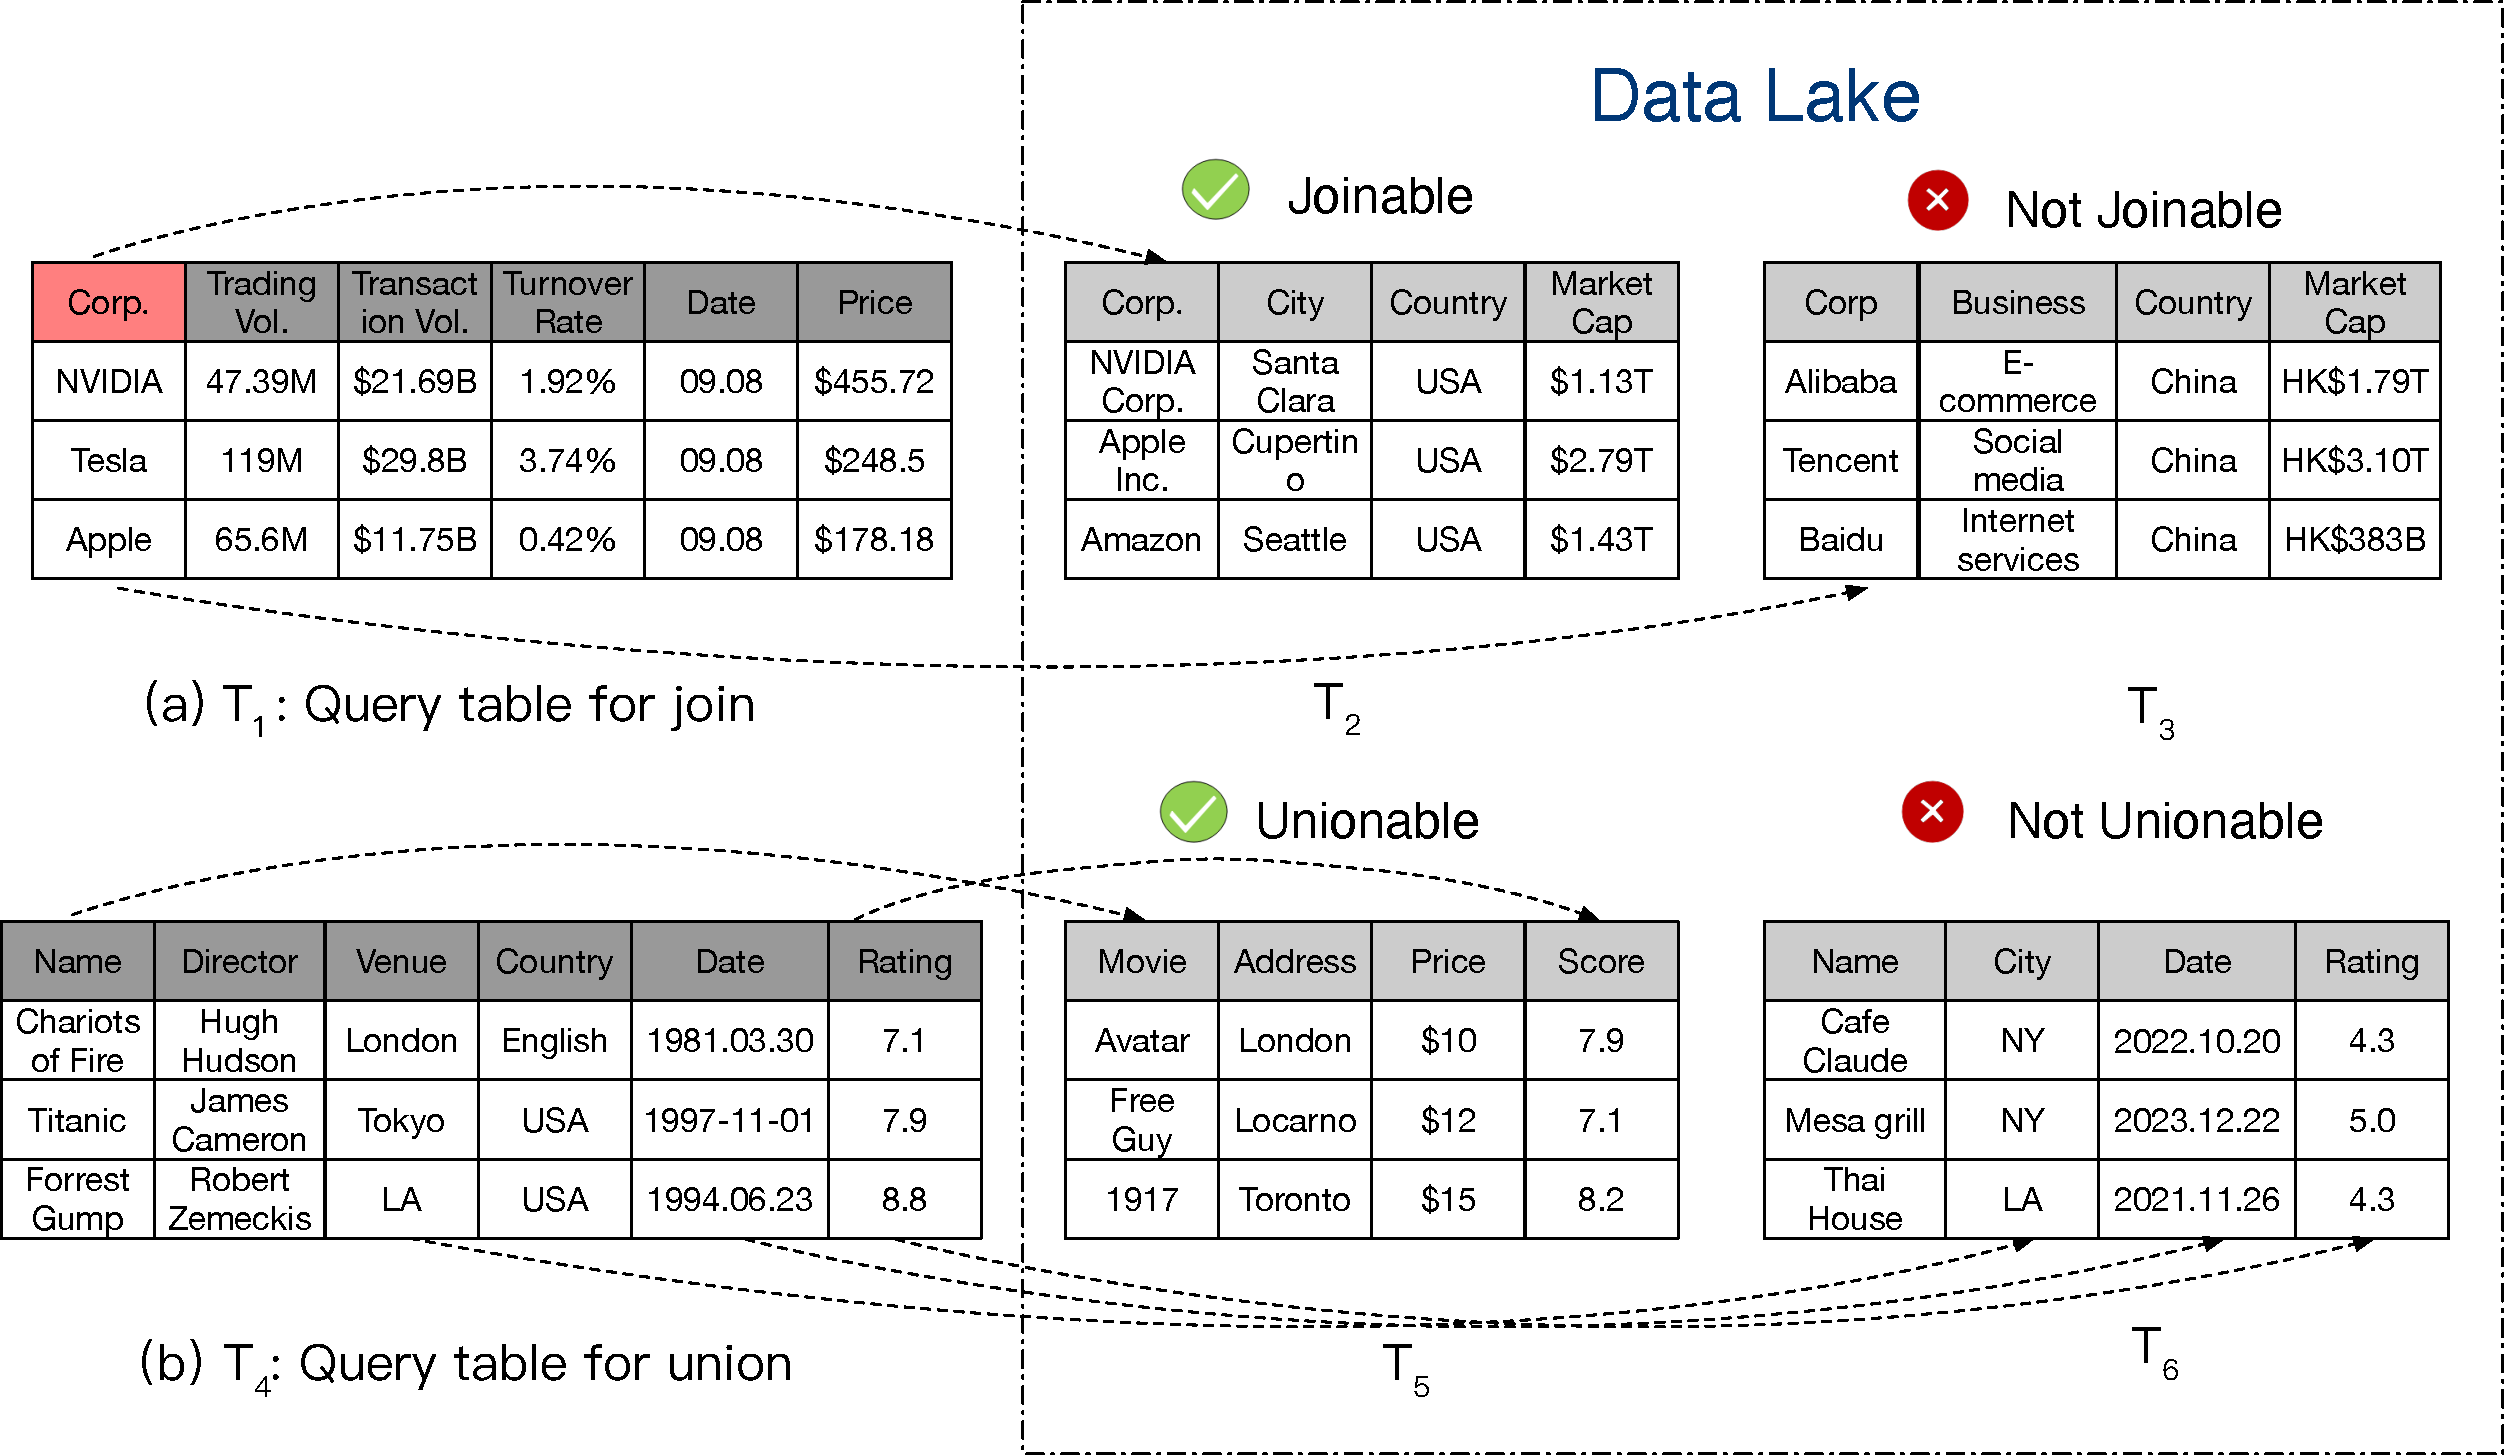
\includegraphics[width=0.8\linewidth]{fig/example.pdf}
	\caption{Table Discovery in Data Lake.}
	\label{fig:example}
\end{figure*}


From the above examples, we can see that table discovery from the data lake is a non-trivial task we should consider (1) the semantic schema similarity of columns, (2) the (semantic) overlappings between columns as well as the (3) contextual information of all columns in a table.
What's more, as the data lake is always large-scale, the efficiency is also a challenging problem. Despite its importance and hardness, existing approaches have still not been evaluated  sufficiently due to the lack of a comprehensive benchmark.  In retrospect, benchmarks have played a significant role
in spawning the boom in different research communities, such as
TPC benchmarks~\cc{\cite{}} for the database community, ImageNet~\cc{\cite{}} for computer vision tasks, and GLUE~\cc{\cite{}} for natural language processing tasks.



\nan{
\bi
	\item Intro
	\be
		\item Sec~1 Add a table or several tables to compare the number of tables/queries supported by your benchmark and others'. 
		\item Easy-to-use APIs: maybe you can give examples for designed unified APIs, saying learned from Hugging Face. They can easily compare different methods. 
		\item Leaderboard.
	\ee
	\item Sec~3 Benchmark design: align with the revised intro
	\item Sec~4 Statistics of datasets, Sec~5 Statistics of queries -- they can be merged if each section is short
	\item Annotation process
	\item API design can be pushed before ``Analyzing benchmark results''
\ei
}




\noindent \textbf{Existing Benchmarks.}  
TUS~\cite{TUS} first builds a benchmark for table union search, which contains around 5,000 tables (from OpenData) in the data lake, among which 1,000 queries are selected as query tables with ground truth. 
Santos~\cite{Santos} improves the TUS benchmark by additionally labeling column-to-column relations to consider more semantics, but it is just for table union search with around 10,100 data lake tables and 80 query tables.
Josie~\cite{Josie} is a join search benchmark that uses two data lakes. One is the same with TUS, and the other is sampled from the Web Table, with 1,000 query columns respectively. 
Valentine~\cite{valentine} evaluates multiple schema matching techniques to solve table discovery tasks, using several hundreds of tables to match pairs of tables. A recent Arxiv work~\cite{arxiv} focuses on evaluating table pretraining methods for table discovery tasks, with the goal of improve downstream machine learning tasks. 

\noindent \textbf{Challenges.} Overall, benchmarking table discovery in data lake faces several major challenges.

\noindent (1) [\textit{Data/Query Coverage}] The effectiveness and efficiency of table discovery largely rely on the characteristics of datasets, like the data lake scale, average column/instance number per table etc. Also, different query  characteristics also lead to different performance, such as query column/table size,  query column type,  result size etc. 

\noindent (2) [\textit{Ground Truth Labeling}] 
 Most existing benchmarks have limited number of queries,  mainly because it is rather expensive to label the ground truth (tables  that can join/union with query in data lake) for each query table. Hence, it is non-trivial to create sufficient queries with ground truth to evaluate different table search approaches.

\noindent (3) [\textit{Solution Coverage}] 
Recently, several unionable/joinable table search methods have been proposed, but there lacks of a thorough comparison over these methods.

\noindent (4) [\textit{User-friendly Interface for Benchmark Usage}] Existing benchmarks just provide datasets, queries and ground truth, which is not very user-friendly if a user wants to
run different algorithms over these benchmarks.


To address the above challenges, in this paper, we create a comprehensive benchmark \sys for table search in data lake.

 First, we collect 3 TB tables from multiple sources, including OpenData, WebTable, and a domain-specific dataset as the data lakes, based on which we evaluate different the table union/join search approaches. These datasets have diverse characteristics. For example, Web table has a large number of tables (XXX) but each has a small size. In contrast, each table in OpenData is quite large (XXX), but the number is smaller than that of WebTable. 
 
 
Second, we create sufficient and diverse queries using two approaches. 
One is to split big tables in data lake into small ones, put these small tables into the data lake and they can be naturally joined or unioned. Hence, when these small tables serve as queries, the ground truth is automatically derived. 
The other one is that we directly use real tables from the data lake as queries, which indicates that we have to spend much efforts labeling ground truth for them.
To better improve the labeling accuracy and human efforts, we design a candidate generation strategy to improve the recall and implement a labeling platform for this task.   

Third, we evaluate various approaches~\cc{\cite{}}, including techniques like schema matching, local sensitive hash,  pre-trained language models etc. for joinable/unionable table search on our benchmark datasets, so as to provide meaningful insights for scalability and accuracy of different approaches on different datasets.

Fourth, we implement an easy-to-use API, based on which a user can conveniently (1) profile the benchmark datasets from different perspectives;
(2) issue join/union table search through few lines of python code;
(3) compare with multiple state-of-the-art discovery algorithms in one line. 

To summarize, we make the following contributions.

\noindent (1) We build a comprehensive benchmark, \sys, for table discovery in data lake, including large-scale datasets, sufficient and various queries, as well as thorough evaluation.  

\noindent (2) We collect more than 3 TB real tables from multiple sources, indexing them with different strategies for table search with different approaches.  

\noindent (3) We create various query tables covering different characteristics, and accurately label ground truth for them.

\noindent (4) We evaluate and analyze multiple state-of-the-art joinable/unionable table search approaches using these created queries on the benchmark datasets.

\noindent (5) We build a use-friendly API to well support table search in data lakes. 

  
